\documentclass[11pt]{article}
\usepackage[margin=1in]{geometry}
\usepackage{graphicx}
\usepackage{booktabs}
\usepackage{hyperref}
\usepackage{amsmath}

\title{HybridCamera: A Weiqi-Board Multimodal Scientific Detector Concept}
\author{Lachlan Chen Research Workspace}
\date{\today}

\begin{document}
\maketitle

\begin{abstract}
HybridCamera is a staged detector concept that combines a central high-dynamic-range single-pixel bucket detector, alternating event and frame-mode tiles, and an optional spectral branch on one synchronized board. The goal is not to immediately fabricate a monolithic event-imager ASIC. The practical first target is a modular board that can be validated with optical scenes, then adapted to NanoMi-style electron microscopy experiments where sparse, high-speed, high-dynamic-range detection is valuable.
\end{abstract}

\section{Motivation}

Frame cameras provide readable texture but waste bandwidth and blur fast dynamics. Event cameras provide sparse temporal contrast with microsecond-class timing but lack static texture and absolute intensity. Single-pixel imaging provides high sensitivity, dynamic range, spectral flexibility, and compressed-sensing compatibility, but needs coded measurements or scan structure. HybridCamera treats these as complementary measurements of the same scene or microscope scan.

The closest architectural precedents are DVS and DAVIS sensors. Lichtsteiner, Posch, and Delbruck demonstrated an asynchronous temporal-contrast sensor with 120 dB dynamic range and 15 us latency. DAVIS later combined DVS events and active-pixel frames in the same pixel array by sharing a photodiode. The proposed board-level design borrows the hybrid idea but keeps each modality modular enough for laboratory iteration.

\section{Weiqi-Board Layout}

The physical concept is a square detector board with a central bucket detector and alternating event/frame tiles around it. The pattern is inspired by a Weiqi board: neighboring positions deliberately hold different capabilities instead of identical pixels.

\begin{figure}[h]
\centering
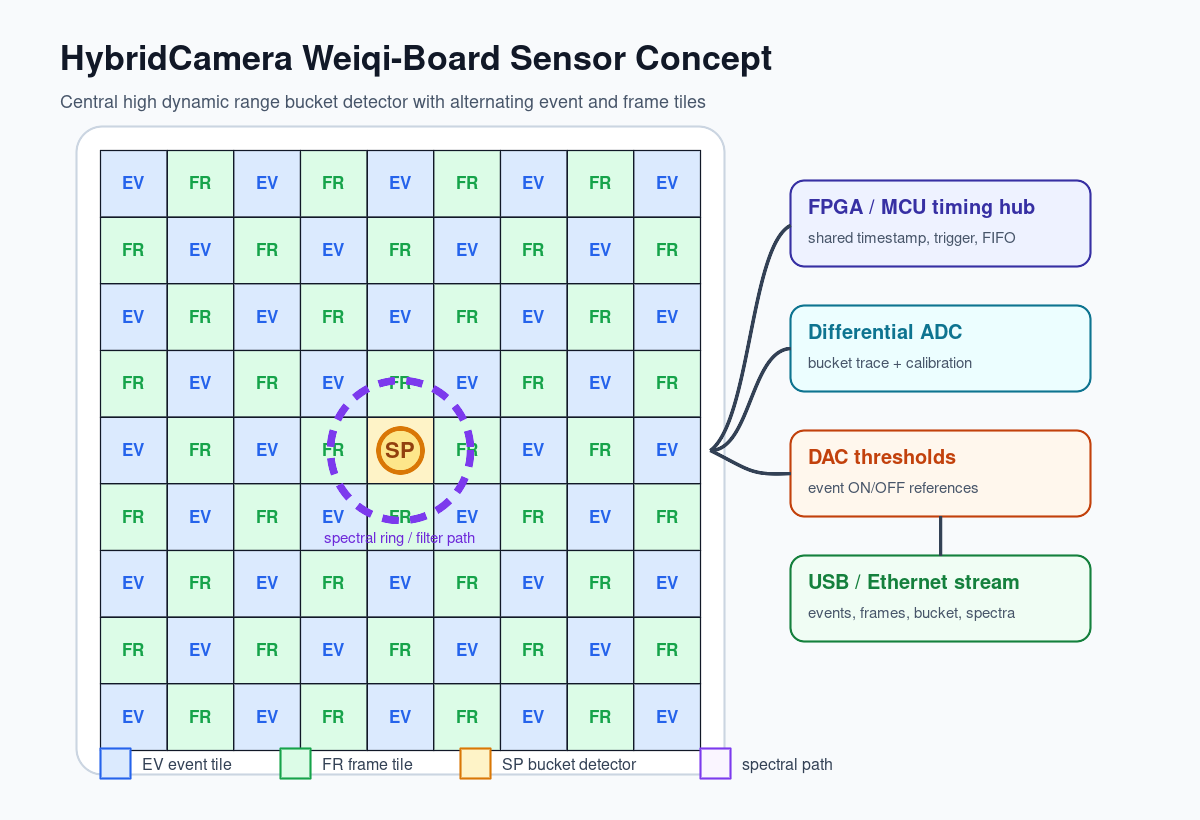
\includegraphics[width=0.95\linewidth]{../figures/hybrid_board_layout.png}
\caption{Deterministic board layout diagram. EV tiles provide sparse temporal events, FR tiles provide frame texture, SP is the central bucket detector, and the dashed ring denotes a possible spectral/filter path.}
\end{figure}

\IfFileExists{../figures/aginti/hybrid-camera-concept.png}{
\begin{figure}[h]
\centering
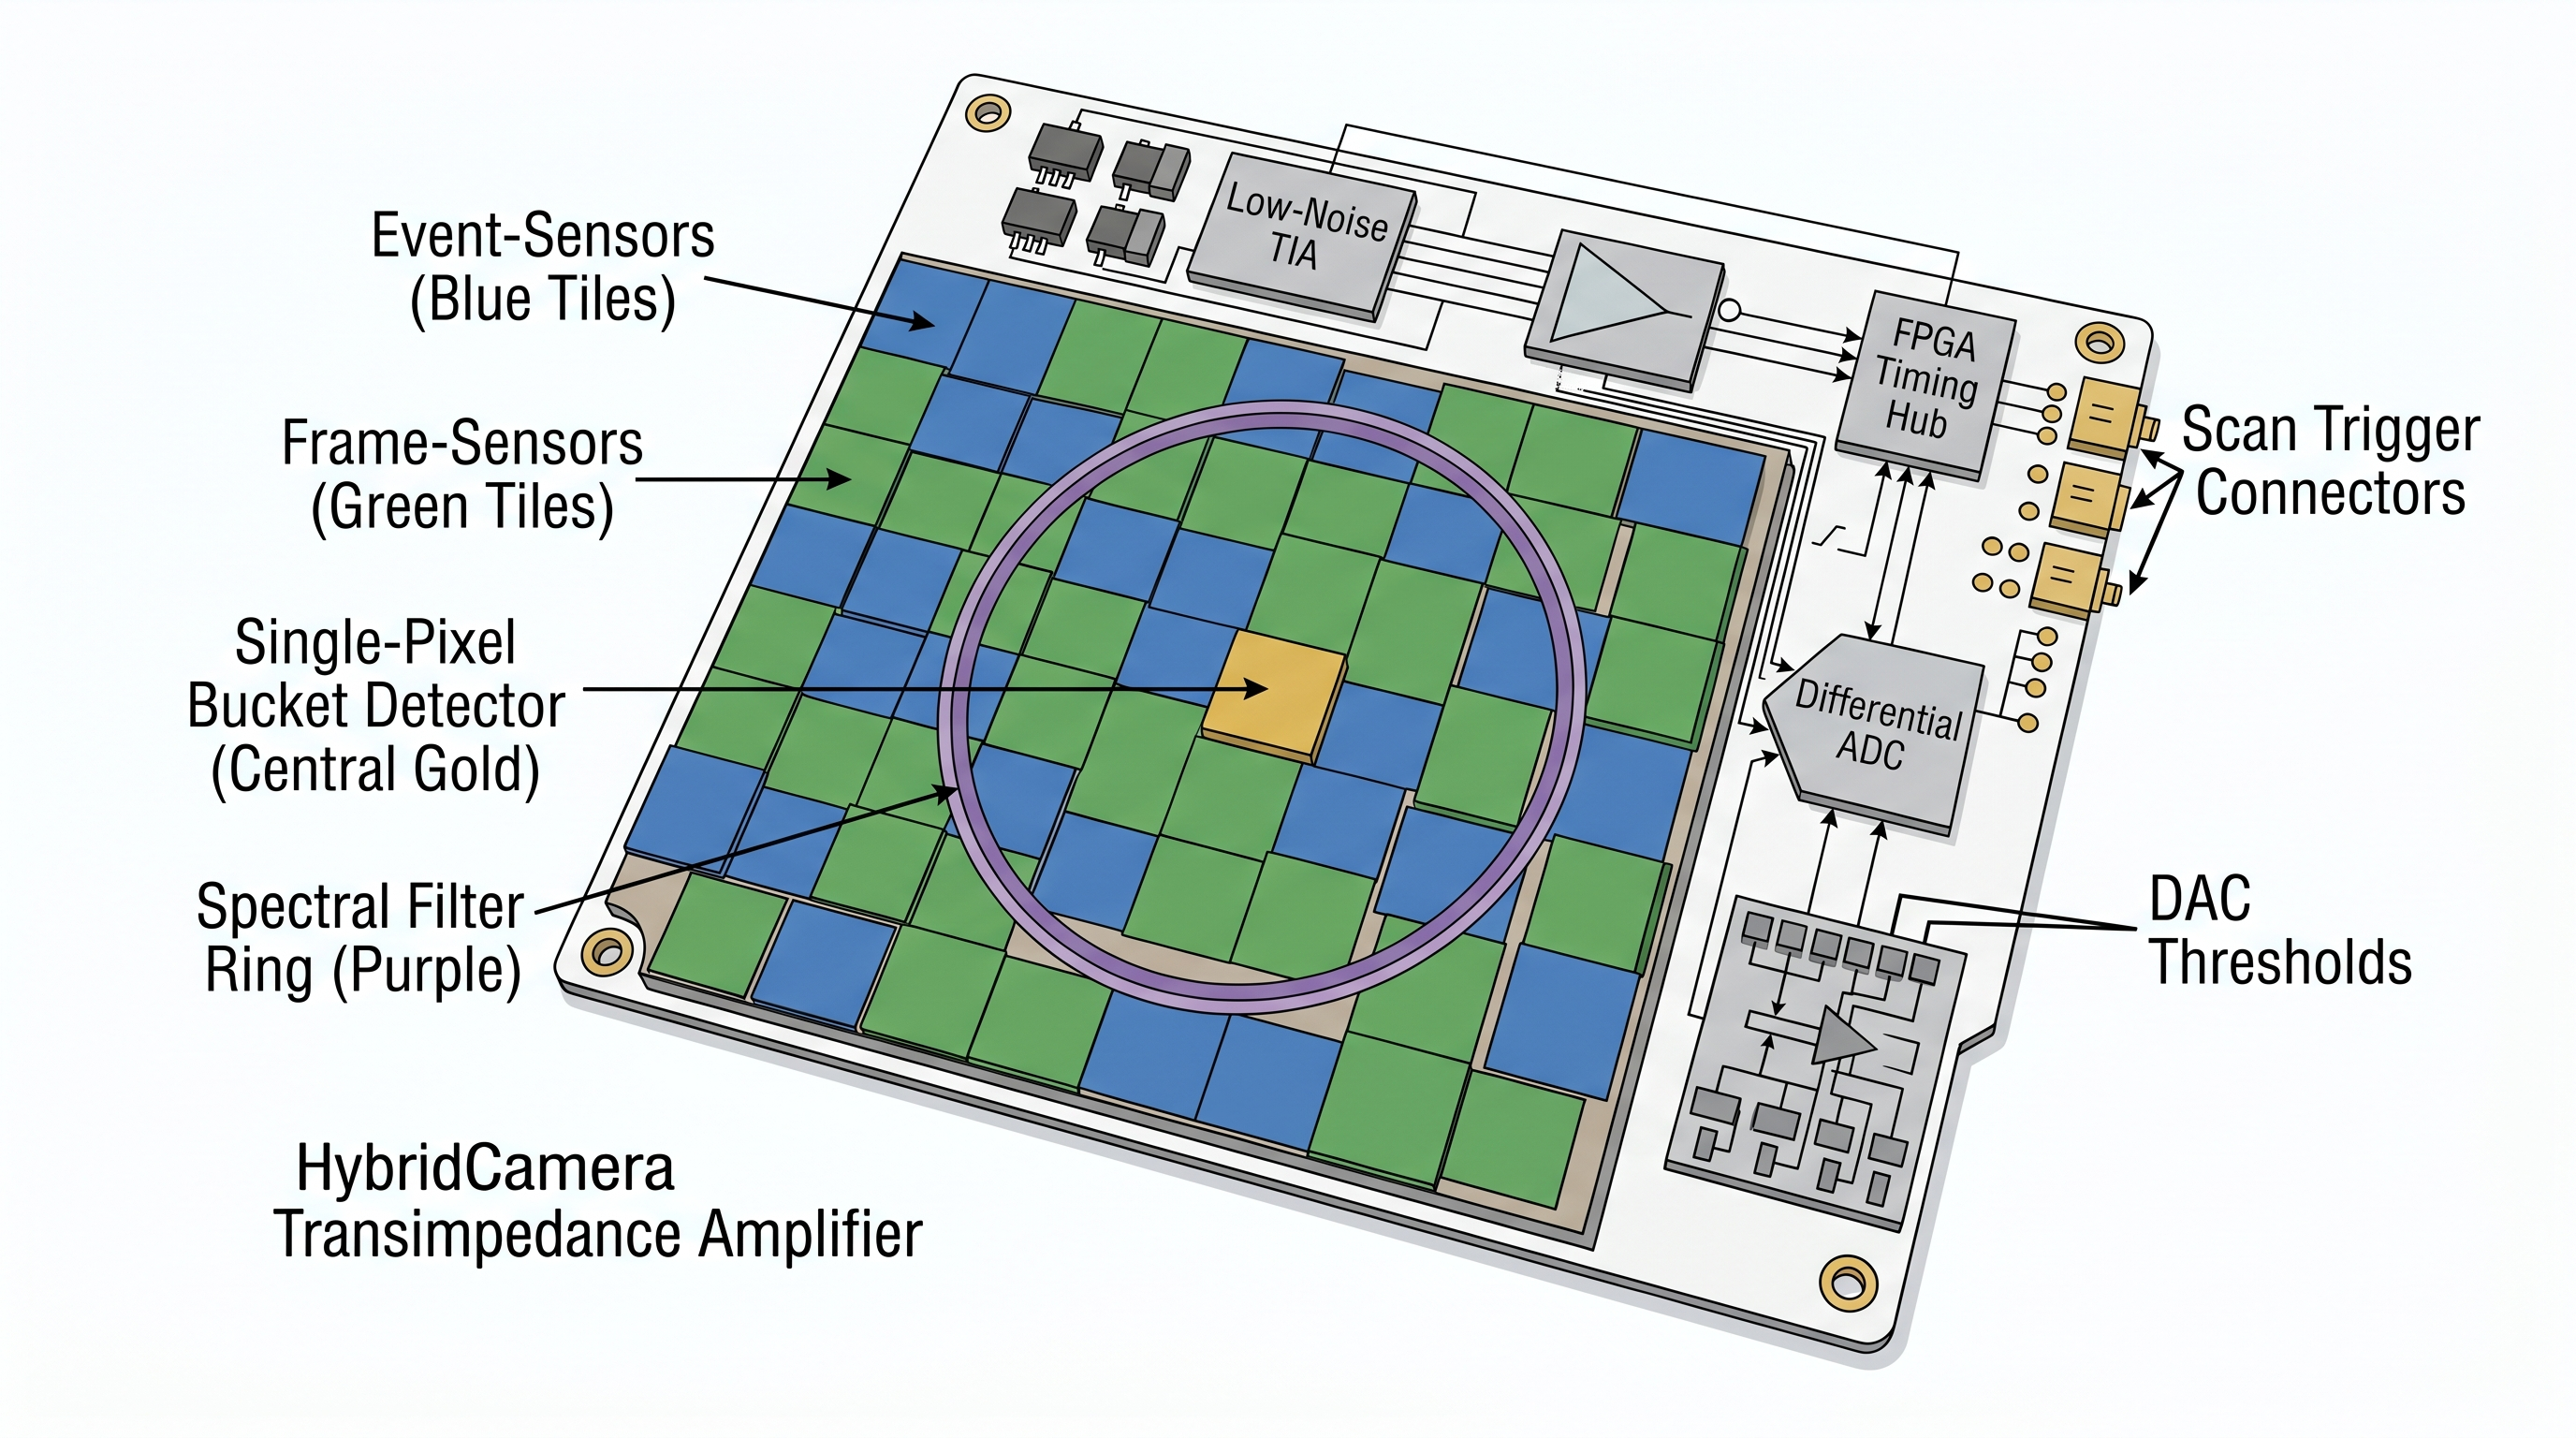
\includegraphics[width=0.95\linewidth]{../figures/aginti/hybrid-camera-concept.png}
\caption{AgInTi-generated concept image for the hybrid board and laboratory setup.}
\end{figure}
}{}

\section{Electronics}

The central bucket detector should use a low-noise transimpedance amplifier (TIA). The detector and op-amp input must be placed close together, with a guarded summing node, selectable feedback resistor/capacitor pairs, dark calibration, and differential ADC readout. The event path can begin as a tiled comparator system: sample a detector value, compare current and baseline values against DAC thresholds, apply hysteresis, then timestamp ON/OFF events. The frame path should prefer global-shutter triggering so frame exposure aligns with event and bucket measurements.

\begin{figure}[h]
\centering
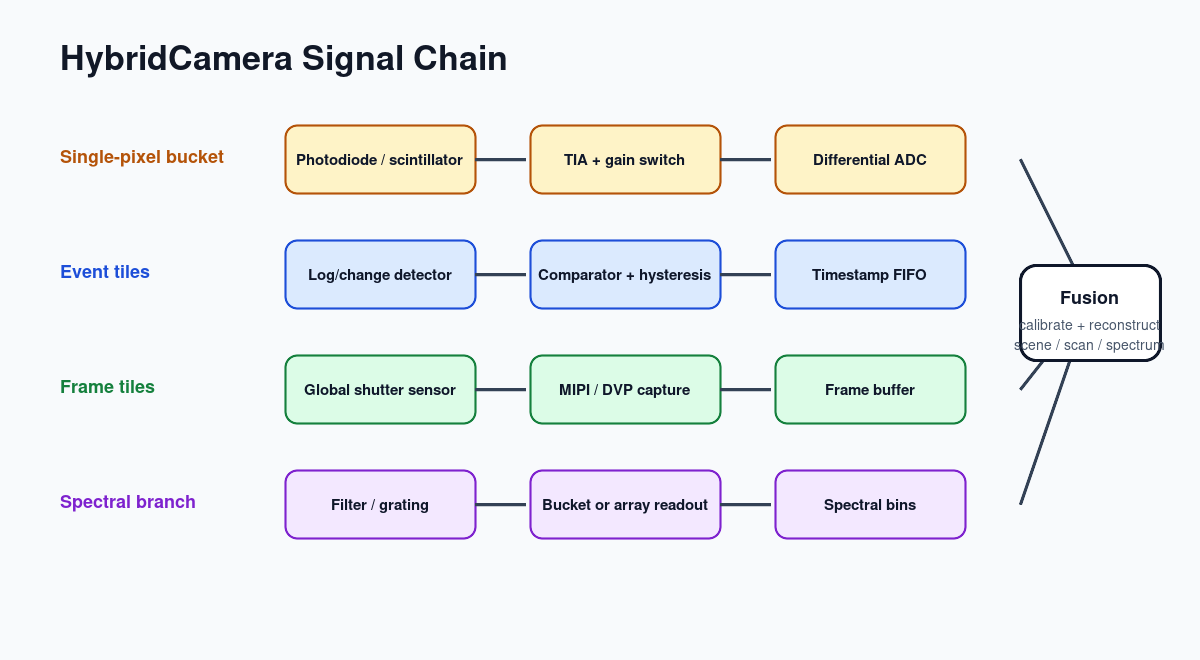
\includegraphics[width=0.95\linewidth]{../figures/hybrid_signal_chain.png}
\caption{Signal-chain view showing how bucket, event, frame, and spectral measurements enter a common reconstruction stack.}
\end{figure}

\section{Wiring and Control}

All streams need one timestamp authority. A small FPGA or high-speed MCU should own the clock, trigger frame exposure, sample the bucket ADC, capture event IRQs or event buses, tag spectral/filter position, and ingest microscope scan or beam-blanking signals. Each record should carry timestamp, source, gain/exposure metadata, and calibration profile ID.

\section{Reconstruction}

Let \(x\) be the latent scene, scan plane, or diffraction plane. The modalities can be represented as
\[
f_k = M_k x + n_f,\quad
y_t = \phi_t^T x + n_y,\quad
e_i = (u_i,v_i,t_i,p_i),\quad
s_\ell = H_\ell x + n_s.
\]
A baseline offline objective is
\[
\min_x \|M_f x - f\|_2^2
+ \alpha\|\Phi x - y\|_2^2
+ \beta E_{\mathrm{event}}(x,e)
+ \gamma TV(x)
+ \eta\|H x - s\|_2^2.
\]
Frame data anchors texture and geometry, events enforce high-speed temporal consistency, bucket measurements constrain dynamic range and saturation, and spectral measurements separate material or wavelength-dependent contrast.

\section{Prototype Plan}

\begin{tabular}{lll}
\toprule
Stage & Hardware & Success criterion \\
\midrule
0 & Frame camera, event camera, photodiode/TIA & synchronized raw streams \\
1 & DIY 4x4 or 8x8 comparator tile & stable ON/OFF events \\
2 & Integrated board with bucket center & calibrated multimodal reconstruction \\
3 & Microscope scan integration & scan-synchronous detector images \\
\bottomrule
\end{tabular}

\section{Conclusion}

The most useful next step is a modular PCB and simulation stack, not a custom ASIC. Once the board-level timebase, data format, TIA performance, event thresholds, and reconstruction objective are stable, the project can decide which sensing functions deserve integration into a custom tile or chip.

\begin{thebibliography}{9}
\bibitem{dvs} P. Lichtsteiner, C. Posch, and T. Delbruck, ``A 128x128 120 dB 15 us Latency Asynchronous Temporal Contrast Vision Sensor,'' IEEE JSSC, 2008.
\bibitem{survey} G. Gallego et al., ``Event-Based Vision: A Survey,'' IEEE TPAMI, 2022.
\bibitem{davis} C. Brandli et al., ``A 240x180 130dB 3us Latency Global Shutter Spatiotemporal Vision Sensor,'' 2014.
\bibitem{singlepixel} M. P. Edgar, G. M. Gibson, and M. J. Padgett, ``Principles and prospects for single-pixel imaging,'' Nature Photonics, 2019.
\bibitem{edi} L. Pan et al., ``Bringing a Blurry Frame Alive at High Frame-Rate with an Event Camera,'' CVPR, 2019.
\bibitem{nanomi} M. Malac et al., ``NanoMi: an open source electron microscope hardware and software platform,'' 2022.
\bibitem{timepix} D. Jannis et al., ``Event driven 4D STEM acquisition with a Timepix3 detector,'' 2021.
\end{thebibliography}

\end{document}
